\let\negmedspace\undefined
\let\negthickspace\undefined
\documentclass[journal]{IEEEtran}
\usepackage[a5paper, margin=10mm, onecolumn]{geometry}
\usepackage{lmodern} % Ensure lmodern is loaded for pdflatex
\usepackage{tfrupee} % Include tfrupee package

\setlength{\headheight}{1cm} % Set the height of the header box
\setlength{\headsep}{0mm}     % Set the distance between the header box and the top of the text

\usepackage{gvv-book}
\usepackage{gvv}
\usepackage{cite}
\usepackage{amsmath,amssymb,amsfonts,amsthm}
\usepackage{algorithmic}
\usepackage{graphicx}
\usepackage{textcomp}
\usepackage{xcolor}
\usepackage{txfonts}
\usepackage{listings}
\usepackage{enumitem}
\usepackage{mathtools}
\usepackage{gensymb}
\usepackage{comment}
\usepackage[breaklinks=true]{hyperref}
\usepackage{tkz-euclide} 
\usepackage{listings}
\usepackage{gvv}                                        
\def\inputGnumericTable{}                                 
\usepackage[latin1]{inputenc}                                
\usepackage{color}                                            
\usepackage{array}                                            
\usepackage{longtable}                                       
\usepackage{calc}                                             
\usepackage{multirow}                                         
\usepackage{hhline}                                           
\usepackage{ifthen}                                           
\usepackage{lscape}
\begin{document}

\bibliographystyle{IEEEtran}
\vspace{3cm}

\title{10.3.6.1.8}
\author{EE24BTECH11060-Sruthi bijili}
% \maketitle
% \newpage
% \bigskip
{\let\newpage\relax\maketitle}
\textbf{Question:}\\
Solve the following pairs of equations by reducing them to a pair of linear equations:
\begin{align*}
    \frac{1}{3x+y} + \frac{1}{3x-y} &= \frac{3}{4}\\
    \frac{1}{2\brak{3x+y}} - \frac{1}{2\brak{3x-y}} &= \frac{-1}{8}
\end{align*}
\textbf{Solution:}\\
Let's solve this using LU decomposition. First, let's substitute:
\begin{align}
    \frac{1}{3x+y} &= u\\
    \frac{1}{3y-y} &= v
\end{align}

Then our equations become:
\begin{align}
    u + v &= \frac{3}{4} \label{eq1}\\
    \frac{1}{2}u - \frac{1}{2}v &= \frac{-1}{8} \label{eq2}
\end{align}
\begin{align}
    4u + 4v &= 3 \label{eq1}\\
    4u - 4v &= -1 \label{eq2}
\end{align}


This can be written in matrix form as:
\begin{align}
    \myvec{4 & 4 \\ 4& -4}\myvec{u\\v} = \myvec{3\\-1}
\end{align}

Any non-singular matrix can be represented as a product of a lower triangular matrix $L$ and an upper triangular matrix $U$
\begin{align}
	\vec{ A}\vec{x} = \vec{L}\vec{U}\vec{x} = \vec{b}
\end{align}
\textbf{Factorization of LU:}\\
Given a matrix $ \mathbf{A} $ of size $ n \times n $, LU decomposition is performed row by row and column by column. The update equations are as follows: 
\begin{itemize}
    \item Start by initializing $ \mathbf{L} $ as the identity matrix $ \mathbf{L} = \mathbf{I} $ and $ \mathbf{U} $ as a copy of $ \mathbf{A} $.\\
    \item For each column $ j \geq k $, the entries of $ U $ in the $ k $-th row are updated as:
    \begin{align}
        U_{k,j} = A_{k,j} - \sum_{m=1}^{k-1} L_{k,m} \cdot U_{m,j}\quad \forall \quad j \geq k
    \end{align}
    \item For each row $ i > k $, the entries of $ L $ in the $ k $-th column are updated as:
    \begin{align}
        L_{i,k} = \frac{1}{U_{k,k}} \brak{ A_{i,k} - \sum_{m=1}^{k-1} L_{i,m} \cdot U_{m,k}} \quad \forall \quad i > k
    \end{align}
\end{itemize}
By doing the following steps and solving we get :
\begin{align}
	\vec{U}=\myvec{4 & 4\\0 & -8} \\
	\vec{ L} = \myvec{1 & 0\\ 1 & 1}
\end{align}

Now,
\begin{align}
    A = \myvec{4& 4\\4 & -4 } = \myvec{1 & 0\\  1 & 1}\myvec{4 & 4\\0 & -8}
\end{align}

We can solve this using two steps:
\begin{align}
    L\vec{y} = \vec{b}\\
    U\vec{x} = \vec{y}
\end{align}

Using forward substitution:
\begin{align}
    \myvec{1 & 0\\ 1 & 1}\myvec{y_1\\y_2} = \myvec{3\\-1}
\end{align}

This gives:
\begin{align}
    y_1 &= 3\\
    3 + y_2 &= -1\\
    y_2 &= -4
\end{align}

Now using back substitution:
\begin{align}
    \myvec{4 & 4\\0 & -8}\myvec{u\\v} = \myvec{3\\ -4}
\end{align}

This gives:
\begin{align}
      \implies v&=\frac{1}{2}\\
    4u + 2 &= 3\\
    u &= \frac{1}{4}
\end{align}

Therefore:
\begin{align}
    \frac{1}{3x+y} =\frac{1}{4} &\implies 3x+y=4\\
    \frac{1}{3x-y} = \frac{1}{2} &\implies 3x-y =2\\
\end{align}
again by LU decomposition for 
\begin{align}
    \myvec{3 & 1 \\ 3& -1}\myvec{x\\y} = \myvec{4\\2}
\end{align}
By doing the following factorization we get:
\begin{align}
	\vec{U}=\myvec{3 & 1\\0 & -2} \\
	\vec{ L} = \myvec{1 & 0\\ 1 & 1}
\end{align}
Using forward substitution:
\begin{align}
    \myvec{1 & 0\\ 1 & 1}\myvec{y_1\\y_2} = \myvec{4\\2}\\
    \implies y_1 =4\\
    \implies y_2 =-2
\end{align}
Now using back substitution:
\begin{align}
    \myvec{3 & 1\\0 & -2}\myvec{x\\y} = \myvec{4\\ -2}
\end{align}

This gives:
\begin{align}
      \implies y&=1\\
    3x + 1 &= 4\\
    x &= 1
\end{align}

The solution is:
\begin{align}
    \myvec{x\\y} = \myvec{1 \\ 1}
 \end{align}

\begin{figure}[h!]
   \centering
	 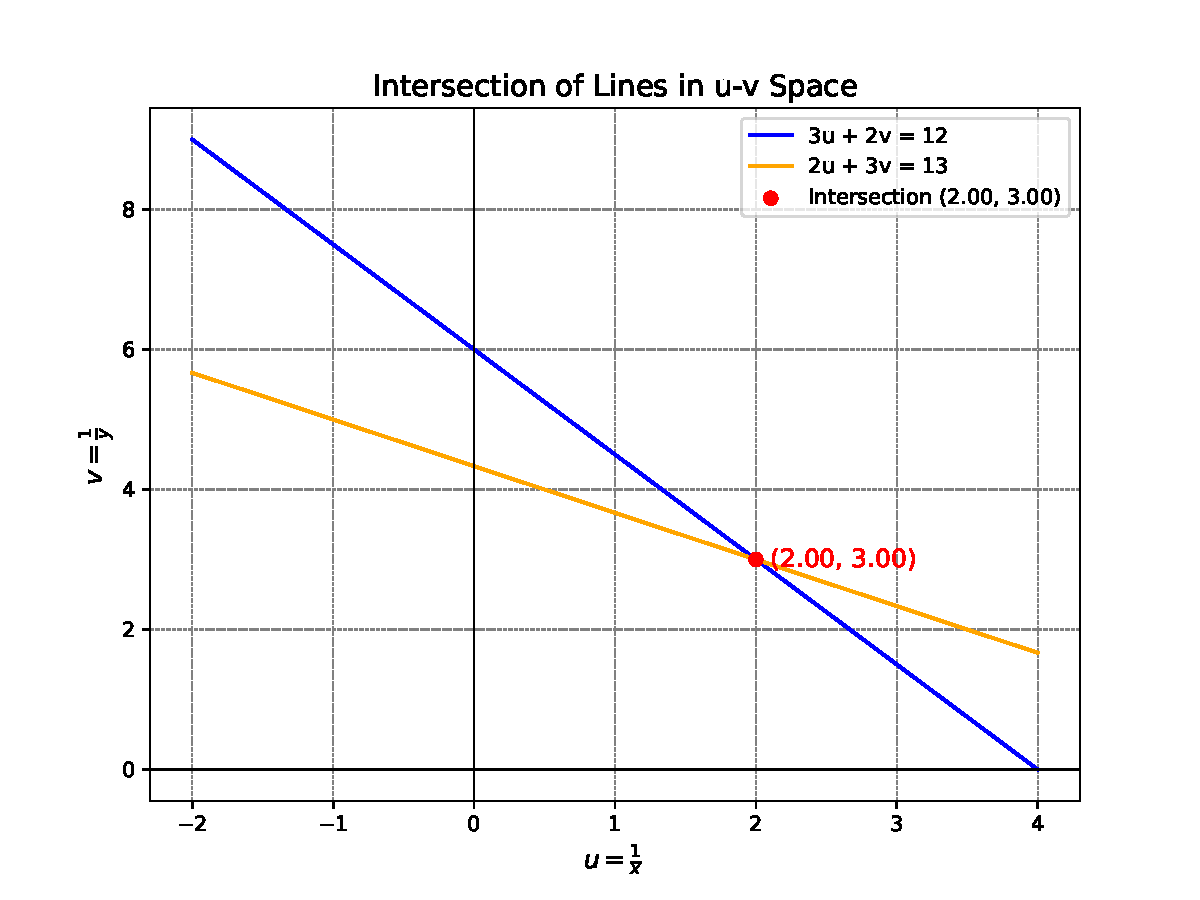
\includegraphics[width=\textwidth]{figs/fig.pdf}
   % Add your figure here if needed
   \caption{Graph of the solution}
\end{figure}





\end{document}
